\subsection{Polarized Proton Collisions}

% factorization
% universality of PDFs and FFs
% partonic cross sections calculable in perturbative QCD

The remainder of this work will focus on extracting information on $\Delta G$
from collisions of polarized proton beams, a task that is made possible by
three key features of the QCD-improved parton model:

\begin{enumerate}
  \item Particle production cross sections can be factorized into a
  convolution of long-range parton distribution functions and fragmentation
  functions and a short-range partonic cross section;
  \item the parton distribution functions and fragmentation functions are
  universal; that is, they can be measured in one reaction and applied to any
  other; and
  \item partonic cross sections in the kinematic range of interest for $\Delta
  G$ studies are calculable using perturbative QCD.
\end{enumerate}

% The QCD-improved parton model allows us to write cross sections in factorized form as a convolution of parton distribution functions, fragmentation functions, and a parton-level cross section.
Ignoring polarization for the moment, we can express the cross section for
inclusive pion production in this framework as a sum over parton flavors
$i,j,k$
%
\begin{equation}
  \sigma^{pp \rightarrow \pi X} = \sum_{i,j,k} \int~dx_1 dx_2 dz~ q_i(x_1) \cdot q_j(x_2) \cdot \sigma^{ij \rightarrow k X}(x_1 p_1,x_2 p_2, p_{\pi}/z) \cdot D_k^\pi(z).
  \label{eqn:factorized}
\end{equation}
%
Here $p_1$ and $p_2$ are the momenta of the colliding proton beams and
$p_{\pi}$ is the momentum of the outgoing pion, while $D_k^{\pi}(z)$ is the
fragmentation function expressing the probability that a parton of flavor $k$
produces a pion carrying a fraction $z$ of the parton's
momentum.\footnote{This interpretation of the fragmentation function is valid
in the simple parton model, and in the QCD improved parton model if one is
working in the light-cone gauge.} Equation \ref{eqn:factorized} is commonly
written using the convolution notation
%
\begin{equation}
  \sigma^{pp \rightarrow \pi X} = \sum_{i,j,k} q_i \otimes q_j \otimes \sigma^{ij \rightarrow kX} \otimes D_k^\pi
\end{equation}.


\begin{equation}
  A_{LL} = \frac{\sum_{f_1,f_2,f}~\Delta f_1 \otimes \Delta f_2 \otimes \sigma^{f_1 f_2 \rightarrow f X'} \hat a_{LL}^{f_1 f_2 \rightarrow f X'} \otimes D_f}{\sum_{f_1,f_2,f}~f_1 \otimes f_2 \otimes \sigma^{f_1 f_2 \rightarrow f X'} \otimes D_f} 
\end{equation}

\begin{equation}
  \hat a_{LL}^{f_1 f_2 \rightarrow f X'} = \frac{\Delta \sigma^{f_1 f_2 \rightarrow f X'}}{\sigma^{f_1 f_2 \rightarrow f X'}}
\end{equation}

\begin{figure}\begin{center}
  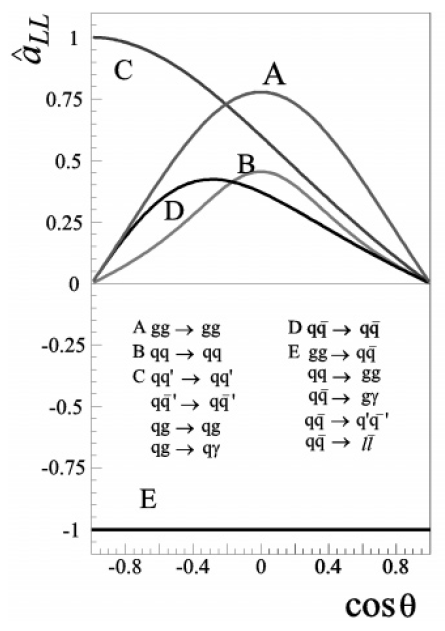
\includegraphics[width=0.5\textwidth]{figures/partonic_asymmetry}
  \caption{Lowest-order analyzing powers for various partonic subprocesses
  present in polarized proton collisions \cite{Bunce:2000uv}.}
\end{center}\end{figure}
